% 13FORGE V3 — WORLD MANDALA TOPOLOGY (PaTeX / LaTeX TikZ Specification)
% Authoritative Declarative Geometry: 13 Zones, +5 mod 12 Quincunx Traversal
\documentclass[tikz,border=10pt]{standalone}
\usepackage{tikz}
\usetikzlibrary{calc,shapes,arrows.meta,decorations.markings}

\begin{document}
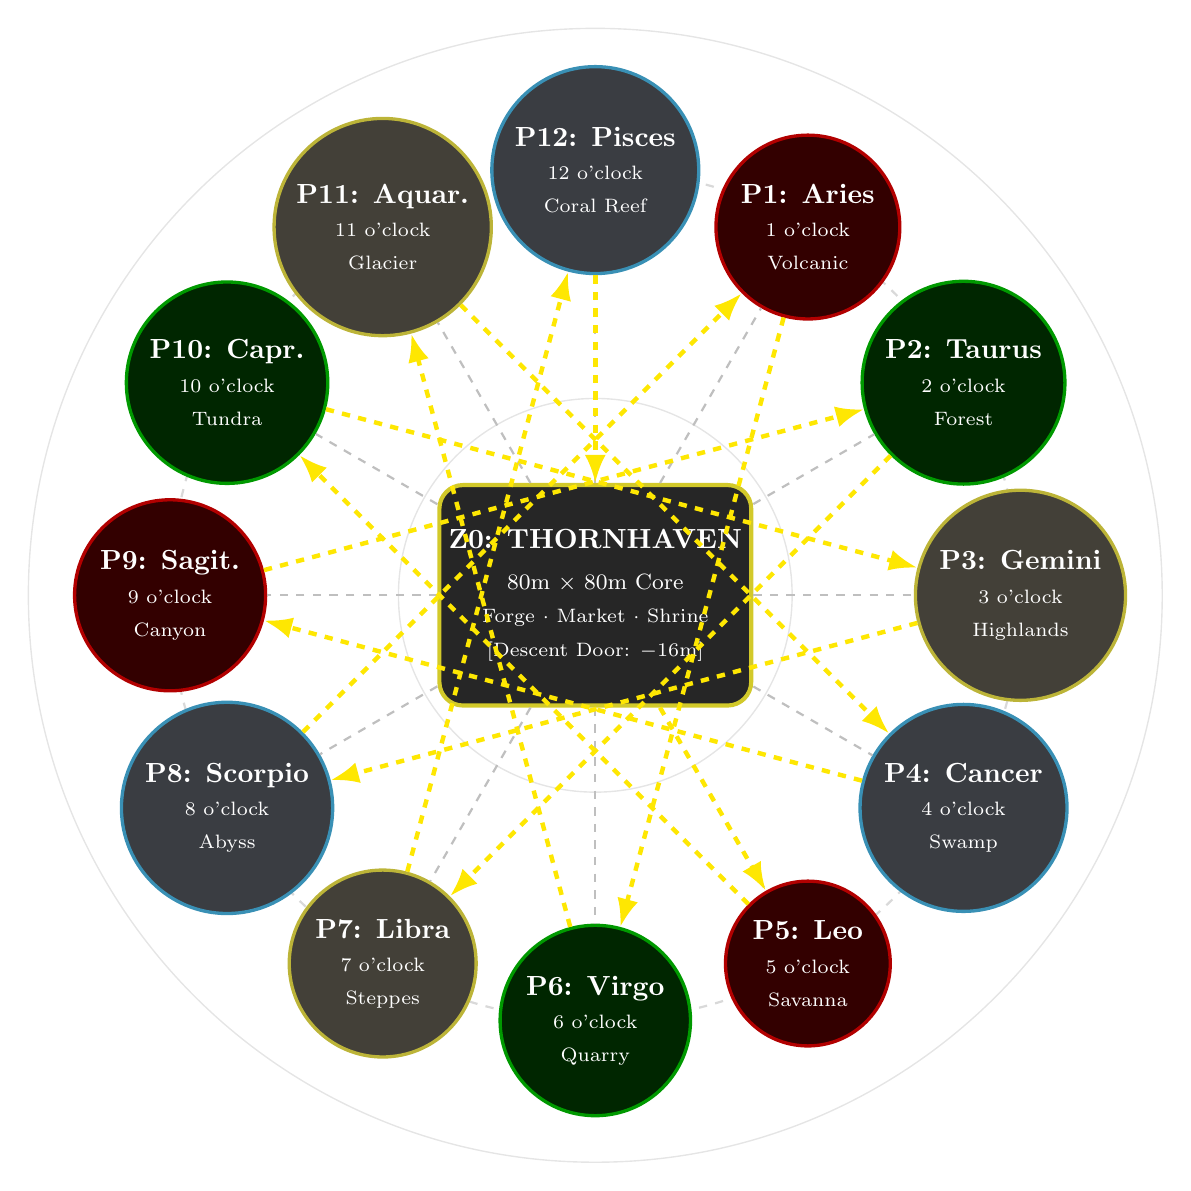
\begin{tikzpicture}[
    scale=1.0,
    >=Latex,
    % Styling for Element Types
    hub/.style={rectangle, rounded corners=3mm, minimum size=2.8cm, draw=yellow!80!black, line width=1.5pt, fill=black!85, text=white, align=center},
    fire/.style={circle, minimum size=1.8cm, draw=red!70!black, line width=1.2pt, fill=red!20!black, text=white, align=center},
    earth/.style={circle, minimum size=1.8cm, draw=green!60!black, line width=1.2pt, fill=green!15!black, text=white, align=center},
    air/.style={circle, minimum size=1.8cm, draw=yellow!70!black, line width=1.2pt, fill=yellow!15!black, text=white, align=center},
    water/.style={circle, minimum size=1.8cm, draw=cyan!70!black, line width=1.2pt, fill=cyan!15!black, text=white, align=center},
    spoke/.style={dashed, color=gray!50, line width=0.8pt},
    quincunx/.style={color=yellow!90!orange, line width=1.6pt, dashed}
]

    % Background Grid / Concentric Rings
    \draw[gray!20, line width=0.5pt] (0,0) circle (2.5cm);
    \draw[gray!30, line width=0.8pt, dashed] (0,0) circle (5.4cm);
    \draw[gray!20, line width=0.5pt] (0,0) circle (7.2cm);

    % Center Hub Z0
    \node[hub] (Z0) at (0,0) {
        \textbf{Z0: THORNHAVEN}\\[1mm]
        \footnotesize 80m $\times$ 80m Core\\
        \scriptsize Forge $\cdot$ Market $\cdot$ Shrine\\
        \scriptsize [Descent Door: $-16$m]
    };

    % 12 Petal Zones (Radial Placement R = 5.4cm, 30 deg intervals)
    \node[water] (P12) at (90:5.4cm)  {\textbf{P12: Pisces}\\\scriptsize 12 o'clock\\\scriptsize Coral Reef};
    \node[fire]  (P1)  at (60:5.4cm)  {\textbf{P1: Aries}\\\scriptsize 1 o'clock\\\scriptsize Volcanic};
    \node[earth] (P2)  at (30:5.4cm)  {\textbf{P2: Taurus}\\\scriptsize 2 o'clock\\\scriptsize Forest};
    \node[air]   (P3)  at (0:5.4cm)   {\textbf{P3: Gemini}\\\scriptsize 3 o'clock\\\scriptsize Highlands};
    \node[water] (P4)  at (330:5.4cm) {\textbf{P4: Cancer}\\\scriptsize 4 o'clock\\\scriptsize Swamp};
    \node[fire]  (P5)  at (300:5.4cm) {\textbf{P5: Leo}\\\scriptsize 5 o'clock\\\scriptsize Savanna};
    \node[earth] (P6)  at (270:5.4cm) {\textbf{P6: Virgo}\\\scriptsize 6 o'clock\\\scriptsize Quarry};
    \node[air]   (P7)  at (240:5.4cm) {\textbf{P7: Libra}\\\scriptsize 7 o'clock\\\scriptsize Steppes};
    \node[water] (P8)  at (210:5.4cm) {\textbf{P8: Scorpio}\\\scriptsize 8 o'clock\\\scriptsize Abyss};
    \node[fire]  (P9)  at (180:5.4cm) {\textbf{P9: Sagit.}\\\scriptsize 9 o'clock\\\scriptsize Canyon};
    \node[earth] (P10) at (150:5.4cm) {\textbf{P10: Capr.}\\\scriptsize 10 o'clock\\\scriptsize Tundra};
    \node[air]   (P11) at (120:5.4cm) {\textbf{P11: Aquar.}\\\scriptsize 11 o'clock\\\scriptsize Glacier};

    % Radial Spokes from Hub to Petals
    \foreach \node in {P1,P2,P3,P4,P5,P6,P7,P8,P9,P10,P11,P12} {
        \draw[spoke] (Z0) -- (\node);
    }

    % Quincunx Traversal Circulation (+5 mod 12 Path)
    % Z0 -> P5 -> P10 -> P3 -> P8 -> P1 -> P6 -> P11 -> P4 -> P9 -> P2 -> P7 -> P12 -> Z0
    \draw[quincunx, ->] (Z0) -- (P5);
    \draw[quincunx, ->] (P5) -- (P10);
    \draw[quincunx, ->] (P10) -- (P3);
    \draw[quincunx, ->] (P3) -- (P8);
    \draw[quincunx, ->] (P8) -- (P1);
    \draw[quincunx, ->] (P1) -- (P6);
    \draw[quincunx, ->] (P6) -- (P11);
    \draw[quincunx, ->] (P11) -- (P4);
    \draw[quincunx, ->] (P4) -- (P9);
    \draw[quincunx, ->] (P9) -- (P2);
    \draw[quincunx, ->] (P2) -- (P7);
    \draw[quincunx, ->] (P7) -- (P12);
    \draw[quincunx, ->] (P12) -- (Z0);

\end{tikzpicture}
\end{document}
